
\begin{center}
\Huge
Vektorer og trigonometri
\end{center}

\section*{Enhedscirklen}
\stepcounter{section}

Trigonometri omhandler regning med trekanter. Til at regne på trekanter har vi såkaldte trigonometriske funktioner, der relaterer sidelængder og vinkler i retvinklede trekanter. De mest kendte trigonometriske funktioner er I formentlig bekendte med: $\cos(v)$ og $\sin(v)$. Vi vil bruge enhedscirklen til at definere disse funktioner. Enhedscirklen kan ses på Figur \ref{fig:enhed}
\begin{figure}[H]
	\begin{center}
	\begin{tikzpicture}
		\begin{axis}[
			axis lines = center, 
			xmin = -1.4, xmax = 1.4, 
			ymin = -1.4, ymax = 1.4, 
			x = 4cm, y = 4cm,
			minor xtick = {-1.4,-1.2,...,1.2,1.4},
			minor ytick = {-1.4,-1.2,...,1.2,1.4},
			xtick = {-1.6},
			ytick = {-1.6},
			xlabel = $x$, ylabel = $y$
		]
			%Shifted tick labels since unit circle would otherwise be in the way:
			\node[xshift = 5pt, yshift = -10pt] at (axis cs:1,0) {1};
			\node[xshift = -8pt, yshift = 5pt] at (axis cs:0,1) {1};
			%Circle, lines and angle:
			\draw[color = teal, thick] (axis cs:0,0) circle (4cm);
			\draw[thick, color = teal] (axis cs: 0,0) to (axis cs: {cos(45)},{sin(45)});
			\draw[thick, color = teal] (axis cs: 0.2,0) arc (0:45:0.8cm) node[midway, xshift = 5pt, yshift = 2pt] {$v$};
			\draw[dashed, thick, color = teal] (axis cs: {cos(45)},{sin(45)}) to (axis cs: {cos(45)},0);
			\draw[dashed, thick, color = teal] (axis cs: {cos(45)},{sin(45)}) to (axis cs: 0,{sin(45)});
			%Text:
			\node[color = teal, anchor = east, xshift = -2pt] at (axis cs: 0,{sin(45)}) {$\sin(v)$};
			\node[color = teal, anchor = north, yshift = -2pt] at (axis cs: {cos(45)},0 ) {$\cos(v)$};
			\node[color = teal, anchor = south west] at (axis cs: {cos(45)},{sin(45)}) {$P_v$};

		\end{axis}
	\end{tikzpicture}
	\end{center}
	\caption{Definition af $\cos$ og $\sin$ ud fra enhedscirklen}
	\label{fig:enhed}
\end{figure}
Enhedscirklen er en cirkel med centrum i origo og radius $1$. Vi kan bruge enhedscirklen til at definere $\cos$ og $\sin$.
\begin{defn}
Lad $P_v$ være et punkt på enhedscirklen, så vinklen mellem stedvektoren $\vv{OP_v}$ og $x$-aksen er $v$. Så defineres funktionerne $\cos(v)$ og $\sin(v)$ som koordinaterne til $P_v$:
\begin{align*}
P_v = (\cos(v),\sin(v)).
\end{align*}
\end{defn}

\begin{exa}
Det gælder, at $\cos(0) = 1$ og $\sin(0)=0$, da koordinatsættet til $P_0$ er 
\begin{align*}
P_0 = (1,0) = (\cos(0),\sin(0)).
\end{align*}
\end{exa}

Skal vi anvende de trigonometriske funktioner i Maple og vi ønsker at anvende grader, så skal vi skrive
\begin{align*}
	&\texttt{with(Gym):} \\
	&\texttt{Cos(v)} \\	
	&\texttt{Sin(v)}
\end{align*}

\begin{setn}[Idiotformlen]
For enhver vinkel $v$ gælder der, at 
\begin{align*}
 \cos(v)^2 + \sin(v)^2 = 1.
\end{align*}
\end{setn}
\begin{proof}
Opgave
\end{proof}

Tangens er den sidste trigonometriske funktion, vi skal betragte. Denne er defineret som 
\begin{align*}
\tan(v) = \frac{\sin(v)}{\cos(v)}.
\end{align*}


\section*{Retvinklede trekanter}
\stepcounter{section}

\begin{setn}
Lad $ABC$ være en trekant med punkterne $A$,  $B$ og $C$ som hjørner, og lad $C$ være en ret vinkel. Så gælder der for vinklen $v$, der er vinklen i enten hjørnet $A$ eller $B$, at 
\begin{align*}
\cos(v) &= \frac{\textnormal{hosliggende katete}}{\textnormal{hypotenuse}}\\
\sin(v) &= \frac{\textnormal{modstående katete}}{\textnormal{hypotenuse}}\\
\tan(v) &= \frac{\textnormal{modstående katete}}{\textnormal{hosliggende katete}}
\end{align*}
\end{setn}

\subsection*{Opgave 1}
\begin{center}
	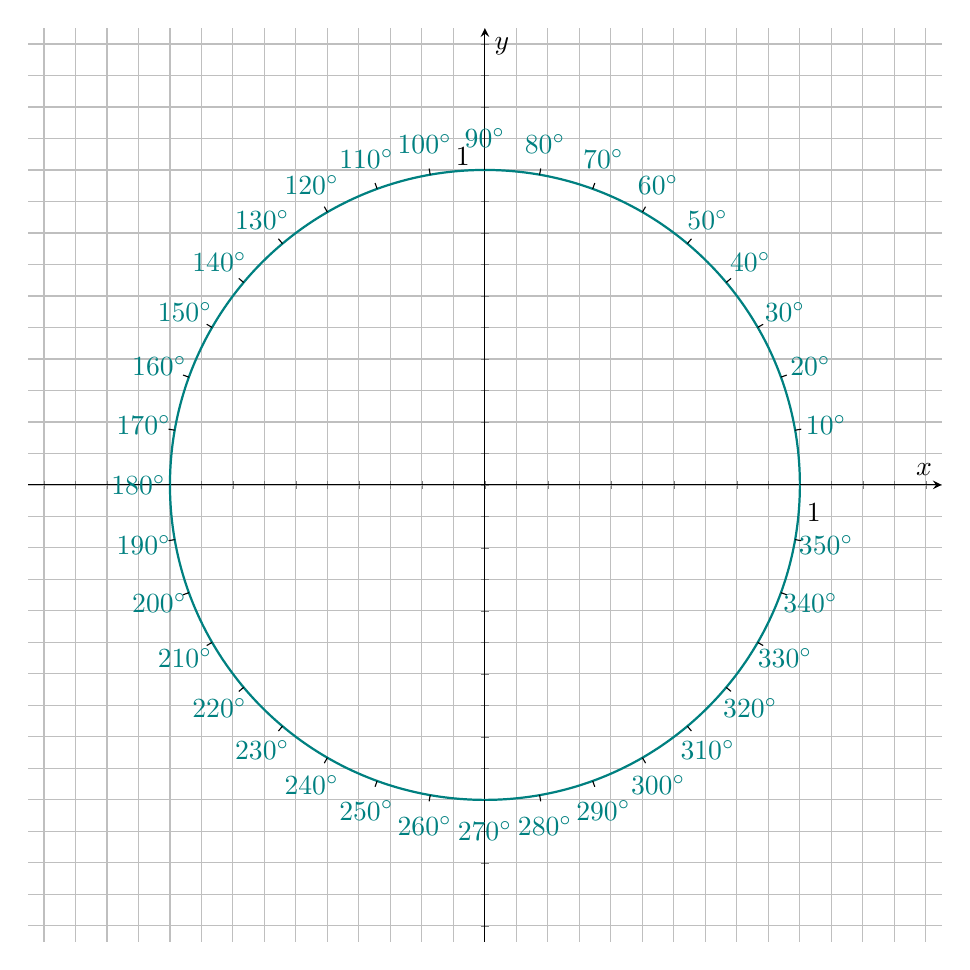
\begin{tikzpicture}
		\begin{axis}[
			axis lines = center, 
			xmin = -1.45, xmax = 1.45, 
			ymin = -1.45, ymax = 1.45, 
			x = 4cm, y = 4cm,
			minor xtick = {-1.4,-1.3,...,1.3,1.4},
			minor ytick = {-1.4,-1.3,...,1.3,1.4},
			grid = both,
			xtick = {-1.6},
			ytick = {-1.6},
			xlabel = $x$, ylabel = $y$
		]
			%Shifted tick labels since unit circle would otherwise be in the way:
			\node[xshift = 5pt, yshift = -10pt] at (axis cs:1,0) {1};
			\node[xshift = -8pt, yshift = 5pt] at (axis cs:0,1) {1};
			\draw[color = teal, thick] (axis cs:0,0) circle (4cm);
			%Ticks on circle 
			\pgfplotsinvokeforeach{0,1,...,35}
			{
				\draw (axis cs: {cos(#1*10)},{sin(#1*10)})-- (axis cs: {1.02*cos(#1*10)},{1.02*sin(#1*10)});
			}
			\pgfplotsinvokeforeach{10,20,...,350}
			{
				\node[color = teal] at (axis cs: {1.10*cos(#1)},{1.10*sin(#1)}) {$#1^\circ$};
			}
		\end{axis}
	\end{tikzpicture}
	\end{center}
Brug enhedscirklen til at aflæse $\cos(v)$ og $\sin(v)$ for følgende vinkler. Tjek dit resultat
\begin{align*}
&1) \ 90  &&2) \ 45   \\
&3) \ 180   &&4) \ 270   \\
&5) \ 60  &&6) \ 120   \\
&7) \ 360  &&8) \ 450   \\
&9) \ 190  &&10) \ 350   \\
&11) \ 300  &&12) \ 220   \\
\end{align*}

\newpage

\subsection*{Opgave 2}

\begin{enumerate}[label=\roman*)]
	\item Aflæs $\sin(60)$ og $\sin(120)$. 
	\item Kan du finde andre vinkler $u$ og $v$, hvor 
	$\sin(u)=\sin(v)?$
	\item Aflæs $\cos(10)$ og $cos(-10)$.
	\item Kan du finde andre vinkler $u$ og $v$, hvor 
	$\cos(u)=\cos(v)?$
	\item Aflæs $\cos(45)$ og $\sin(45)$. 
	\item Kan du finde andre vinkler $v$, så $\cos(v)=\sin(v)$
\end{enumerate}

\subsection*{Opgave 3}
\begin{enumerate}[label=\roman*)]
	\item Brug enhedscirklen til at løse ligningen $\cos(v) = 0.5$
	\item Brug enhedscirklen til at løse ligningen $\sin(v) = 0.8$
	\item Brug enhedscirklen til at løse ligningen $\cos(v) = -0.2$
\end{enumerate}

\subsection*{Opgave 4}
Vi skal bevise idiotformlen. Vi betragter derfor vektoren $\vv{OP_v}$, der går fra origo ud til randen af enhedscirklen.
\begin{enumerate}[label=\roman*)]
	\item Opskriv koordinaterne til vektoren $\vv{OP_v}$.
	\item Brug længdeformlen for vektorer til at opskrive længden af vektoren $\vv{OP_v}$
	\item Udnyt, at du allerede kender længden af $\vv{OP_v}$, og sæt dit udtryk fra ii) lig 
	denne længde. (Vink: Hvad er radius for enhedscirklen?)
	\item Opløft begge sider af lighedstegnet i 2 og sammenlign med idiotformlen. 
\end{enumerate}

\subsection*{Opgave 5}
Brug dit resultat fra Opgave 1 til at bestemme tangens for følgende vinkler
\begin{align*}
&1) \ 0  &&2) \ 45   \\
&3) \ 180   &&4) \ 270   \\
&5) \ 60  &&6) \ 120   \\
&7) \ 360  &&8) \ 450   \\
\end{align*}


\subsection*{Opgave 6}
Brug idiotformlen til at bestemme $\cos(45)$ eksakt.

\subsection*{Opgave 7}
\begin{enumerate}[label=\roman*)]
\item Brug enhedscirklen til at argumentere for, at $\cos(30) = 0.5$.
\item Brug nu denne information samt idiotformlen til at bestemme $\sin(30)$.
\item Brug nu enhedscirklen til at bestemme $\sin(60)$ og $\cos(60)$. 

\end{enumerate}


\subsection*{Opgave 8}
Bestem de ukendte sider og vinkler i følgende trekanter:

\begin{tikzpicture}
\node at (0,0) (1) {$A$};
\node at (5,0) (2) {$C$};
\node at (5,3)(3)	{$B$};
\node at (1.2,0.3) (4)   {\scriptsize $30^\circ$};
\node at (2.5,-0.5)  {$5$};


\draw (1) -- (2);
\draw (2) -- (3);
\draw (3) -- (1);
\end{tikzpicture}

\begin{tikzpicture}
\node at (0,0) (1) {$A$};
\node at (4,0) (2) {$C$};
\node at (4,4) (3)	{$B$};
\node at (1.2,0.3)  {};% {\scriptsize $30^\circ$};
\node at (2,-0.5)  {$3$};
\node at (1.8,2.2)   {$4$};

\draw (1) -- (2);
\draw (2) -- (3);
\draw (3) -- (1);
\end{tikzpicture}


\begin{tikzpicture}
\node at (0,0) (1) {$A$};
\node at (3,0) (2) {$C$};
\node at (3,6) (3)	{$B$};
\node at (1.5,-0.3)  {$3$};
\node at (3.3,3)  {$6$};


\draw (1) -- (2);
\draw (2) -- (3);
\draw (3) -- (1);
\end{tikzpicture}

\subsection*{Opgave 9}
Vi står foran en høj bygning og vil gerne bestemme, hvor høj den er. Vi står 300m fra bygningen og måler, at vinklen mellem jorden og sigtelinjen fra jorden til toppen af bygningen er $25^\circ$.
\begin{enumerate}[label=\roman*)]
\item Hvor langt er der i lige linje fra os til toppen af bygningen?
\item Hvor høj er bygningen?
\end{enumerate}

